\documentclass[12pt]{article}

\usepackage{sbc-template}
\usepackage{graphicx,url}
\usepackage[utf8]{inputenc}
\usepackage[brazil]{babel}
\usepackage{comment}
\usepackage{tabularx}
%\usepackage[latin1]{inputenc}  


\begin{comment}
\sloppy

\title{Instructions for Authors of SBC Conferences\\ Papers and Abstracts}

\author{Luciana P. Nedel\inst{1}, Rafael H. Bordini\inst{2}, Flávio Rech
  Wagner\inst{1}, Jomi F. Hübner\inst{3} }


\address{Instituto de Informática -- Universidade Federal do Rio Grande do Sul
  (UFRGS)\\
  Caixa Postal 15.064 -- 91.501-970 -- Porto Alegre -- RS -- Brazil
\nextinstitute
  Department of Computer Science -- University of Durham\\
  Durham, U.K.
\nextinstitute
  Departamento de Sistemas e Computação\\
  Universidade Regional de Blumenal (FURB) -- Blumenau, SC -- Brazil
  \email{\{nedel,flavio\}@inf.ufrgs.br, R.Bordini@durham.ac.uk,
  jomi@inf.furb.br}
}

\begin{document} 

\maketitle

\begin{abstract}
  This meta-paper describes the style to be used in articles and short papers
  for SBC conferences. For papers in English, you should add just an abstract
  while for the papers in Portuguese, we also ask for an abstract in
  Portuguese (``resumo''). In both cases, abstracts should not have more than
  10 lines and must be in the first page of the paper.
\end{abstract}
     
\begin{resumo} 
  Este meta-artigo descreve o estilo a ser usado na confecção de artigos e
  resumos de artigos para publicação nos anais das conferências organizadas
  pela SBC. É solicitada a escrita de resumo e abstract apenas para os artigos
  escritos em português. Artigos em inglês deverão apresentar apenas abstract.
  Nos dois casos, o autor deve tomar cuidado para que o resumo (e o abstract)
  não ultrapassem 10 linhas cada, sendo que ambos devem estar na primeira
  página do artigo.
\end{resumo}


\section{General Information}

All full papers and posters (short papers) submitted to some SBC conference,
including any supporting documents, should be written in English or in
Portuguese. The format paper should be A4 with single column, 3.5 cm for upper
margin, 2.5 cm for bottom margin and 3.0 cm for lateral margins, without
headers or footers. The main font must be Times, 12 point nominal size, with 6
points of space before each paragraph. Page numbers must be suppressed.

Full papers must respect the page limits defined by the conference.
Conferences that publish just abstracts ask for \textbf{one}-page texts.

\section{First Page} \label{sec:firstpage}

The first page must display the paper title, the name and address of the
authors, the abstract in English and ``resumo'' in Portuguese (``resumos'' are
required only for papers written in Portuguese). The title must be centered
over the whole page, in 16 point boldface font and with 12 points of space
before itself. Author names must be centered in 12 point font, bold, all of
them disposed in the same line, separated by commas and with 12 points of
space after the title. Addresses must be centered in 12 point font, also with
12 points of space after the authors' names. E-mail addresses should be
written using font Courier New, 10 point nominal size, with 6 points of space
before and 6 points of space after.

The abstract and ``resumo'' (if is the case) must be in 12 point Times font,
indented 0.8cm on both sides. The word \textbf{Abstract} and \textbf{Resumo},
should be written in boldface and must precede the text.

\section{CD-ROMs and Printed Proceedings}

In some conferences, the papers are published on CD-ROM while only the
abstract is published in the printed Proceedings. In this case, authors are
invited to prepare two final versions of the paper. One, complete, to be
published on the CD and the other, containing only the first page, with
abstract and ``resumo'' (for papers in Portuguese).

\section{Sections and Paragraphs}

Section titles must be in boldface, 13pt, flush left. There should be an extra
12 pt of space before each title. Section numbering is optional. The first
paragraph of each section should not be indented, while the first lines of
subsequent paragraphs should be indented by 1.27 cm.

\subsection{Subsections}

The subsection titles must be in boldface, 12pt, flush left.

\section{Figures and Captions}\label{sec:figs}


Figure and table captions should be centered if less than one line
(Figure~\ref{fig:exampleFig1}), otherwise justified and indented by 0.8cm on
both margins, as shown in Figure~\ref{fig:exampleFig2}. The caption font must
be Helvetica, 10 point, boldface, with 6 points of space before and after each
caption.

\begin{figure}[ht]
\centering
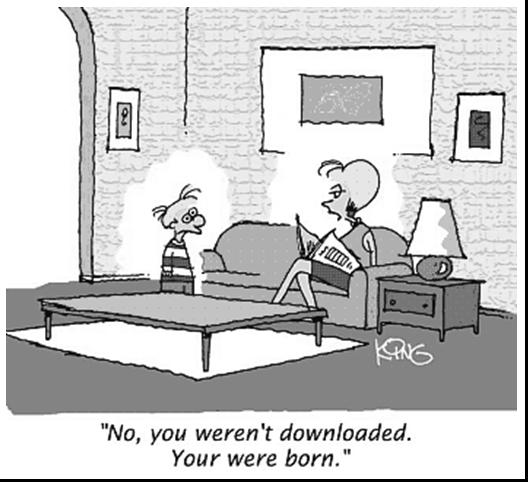
\includegraphics[width=.5\textwidth]{fig1.jpg}
\caption{A typical figure}
\label{fig:exampleFig1}
\end{figure}

\begin{figure}[ht]
\centering
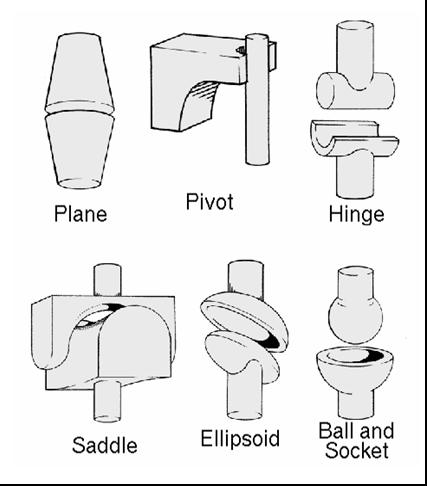
\includegraphics[width=.3\textwidth]{fig2.jpg}
\caption{This figure is an example of a figure caption taking more than one
  line and justified considering margins mentioned in Section~\ref{sec:figs}.}
\label{fig:exampleFig2}
\end{figure}

In tables, try to avoid the use of colored or shaded backgrounds, and avoid
thick, doubled, or unnecessary framing lines. When reporting empirical data,
do not use more decimal digits than warranted by their precision and
reproducibility. Table caption must be placed before the table (see Table 1)
and the font used must also be Helvetica, 10 point, boldface, with 6 points of
space before and after each caption.

\begin{table}[ht]
\centering
\caption{Variables to be considered on the evaluation of interaction
  techniques}
\label{tab:exTable1}
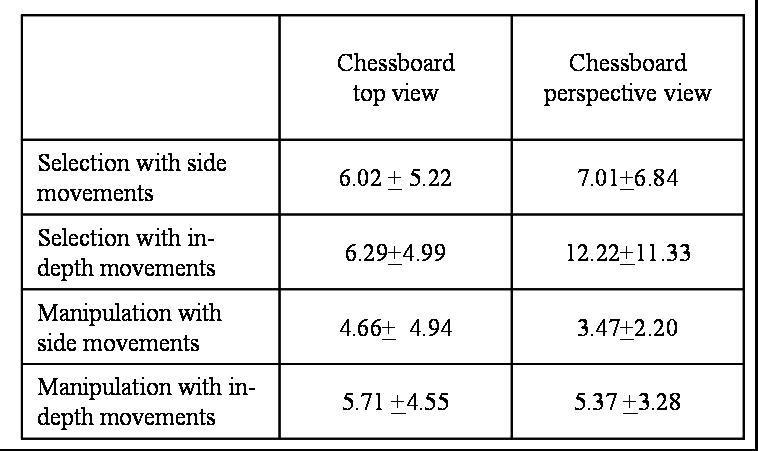
\includegraphics[width=.7\textwidth]{table.jpg}
\end{table}

\section{Images}

All images and illustrations should be in black-and-white, or gray tones,
excepting for the papers that will be electronically available (on CD-ROMs,
internet, etc.). The image resolution on paper should be about 600 dpi for
black-and-white images, and 150-300 dpi for grayscale images.  Do not include
images with excessive resolution, as they may take hours to print, without any
visible difference in the result. 

\section{References}

Bibliographic references must be unambiguous and uniform.  We recommend giving
the author names references in brackets, e.g. \cite{knuth:84},
\cite{boulic:91}, and \cite{smith:99}.

The references must be listed using 12 point font size, with 6 points of space
before each reference. The first line of each reference should not be
indented, while the subsequent should be indented by 0.5 cm.

\bibliographystyle{sbc}
\bibliography{sbc-template}

\end{document}
\end{comment}

%% =====================================================================
%% MAPA DE CITAÇÕES (substitua depois pelas chaves do seu BibTeX)
%%  [1]  Rajath & Vivian (2026)      Next Sustainability 7, 100311
%%  [2]  Różycki et al. (2025)       Energies 18(11), 2810
%%  [3]  Khan et al. (2026)          Sustainable Environment 12(1)
%%  [4]  Bayoumi et al. (2026)       J. King Saud Univ. CIS 38:304
%%  [5]  Verdecchia et al. (2023)    WIREs DMKD 13(4):e1507
%%  [6]  Lal & You (2025)            Advances in Applied Energy 20:100243
%%  [7]  Oliveira et al. (2026)      Sustainability 18, 1359
%%  [8]  Marmouzi et al. (2026)      Sustainability 18, 4115
%%  [9]  Frimpong (2025)             "What Counts as Green AI..."
%%  [10] Peykani et al. (2026)       Arch. Comput. Methods Eng. 33
%%  [11] Rojahn & Grum (2026)        Inf. Softw. Technol. 198, 108186
%%  [12] Alobid & Szucs (2026)       Next Sustainability 8, 100470
%%  [13] Naser (2026)                Renew. Sustain. Energy Rev. 226, 116231
%%
%% CONVENÇÕES DESTE ARQUIVO
%%  - \cite{n}      -> citação destacada em AZUL NEGRITO (trocar por \cite{chave})
%%  - \inserir{..} -> campo que VOCÊ deve preencher, em VERMELHO NEGRITO
%%  - \imagem{..}  -> espaço de figura, com o que inserir dentro dele
%% =====================================================================

\usepackage{sbc-template}
\usepackage{graphicx,url}
\usepackage[utf8]{inputenc}
\usepackage[brazil]{babel}
\usepackage{comment}
\usepackage{xcolor}
\usepackage{float}

% ---- Macros de destaque (REMOVER/AJUSTAR ao finalizar) ----
\newcommand{\cit}[1]{\textbf{\textcolor{blue}{[#1]}}}
\newcommand{\inserir}[1]{\textbf{\textcolor{red}{[INSERIR: #1]}}}
\newcommand{\imagem}[2]{%
  \begin{center}
  \fbox{\parbox{0.85\textwidth}{\centering\vspace{1.2cm}
  \textbf{\textcolor{red}{[ESPAÇO DA FIGURA: #1]}}\\[4pt]
  \textcolor{red}{O que inserir: #2}\vspace{1.2cm}}}
  \end{center}}

\sloppy

\title{Do Consumo de Energia ao Ciclo de Vida: Definição, Medição e Redução do Impacto Ambiental da Inteligência Artificial}

\author{Mateus de Almeida Souza\inst{1}, Thiago Nascente Borges\inst{1},\\
Moises Ferreira Protazio Bastos\inst{1}, Deivison Oliveira da Silva\inst{1},\\
Jacson Rodrigues Barbosa\inst{1}}

\address{Instituto de Informática (INF) -- Universidade Federal de Goiás (UFG)\\
  Goiânia -- GO -- Brasil\\
  {\small\texttt{mateussouza@discente.ufg.br, thiago\_nascente@discente.ufg.br,}}\\
  {\small\texttt{moisesbastos@discente.ufg.br, deivison@discente.ufg.br,}}\\
  {\small\texttt{jacson\_rodrigues@ufg.br}}
}

\begin{document}

\maketitle

%%\maketitle

\begin{abstract}
  This paper synthesizes thirteen recent reviews on Green AI to examine how the
  environmental impact of artificial intelligence is defined, measured and
  reduced. The analysis shows that the definition has moved from training
  energy to a full life-cycle footprint that includes hardware, water and
  social justice, and that a reduction only counts if it is net, absolute and
  measured within declared boundaries. Techniques at the data, model, hardware
  and operational levels are compared, and the main bottlenecks (inconsistent
  boundaries, proxy metrics, second-hand evidence and rebound effects) are
  discussed. Future directions center on standardized reporting, mandatory
  life-cycle assessment and absolute caps.
\end{abstract}

\begin{resumo}
  Este artigo sintetiza treze revisões recentes sobre Green AI para examinar
  como o impacto ambiental da inteligência artificial é definido, medido e
  reduzido. A análise mostra que a definição migrou da energia do treinamento
  para uma pegada de ciclo de vida completo, que inclui hardware, água e
  justiça social, e que uma redução só é válida se for líquida, absoluta e
  medida em fronteiras declaradas. São comparadas técnicas nos níveis de dados,
  modelo, hardware e operação, e discutidos os principais gargalos (fronteiras
  inconsistentes, métricas indiretas, evidência de segunda mão e efeito
  rebote). As direções futuras giram em torno de relato padronizado, avaliação
  de ciclo de vida obrigatória e tetos absolutos.
\end{resumo}

\section{Introdução}

O uso de inteligência artificial (IA) eleva o consumo de eletricidade, de emissões de carbono e de demanda por água e materiais da infraestrutura que a sustenta \cite{1, 2, 6}. A literatura responde com o conceito de \emph{Green AI}, que se contrapõe à \emph{Red AI}, orientada apenas ao desempenho \cite{1, 4, 10}. Apesar do volume de revisões e dos trabalhos usados em cada, não há consenso sobre o que significa ``reduzir'' o impacto, nem sobre como medi-lo de forma comparável.

Este trabalho reúne treze revisões publicadas entre 2023 e 2026 e busca responder três perguntas: (i) como o impacto ambiental da IA é definido e como essa definição mudou; (ii) como ele é medido; e (iii) que técnicas são propostas para reduzi-lo.

\section{Método}

Inicialmente, usando a \emph{string de busca} \emph{"Green AI"}, na base de dados \emph{Scopus}, foram selecionados, com data de corte em setembro de 2026, todas as revisões que apresentavam o termo \emph{"Green AI"} no Título, \emph{Abstract}, ou como palavra chave; resultando em 43 trabalhos. Desses, apenas 13 tratavam, de forma inequívoca, sobre \emph{"Green AI"}. Por exemplo, embora o trabalho \cite{16} estivesse contido entre os 43 iniciais, ele não trata a \emph{Green AI} no sentido estrito de tornar o treinamento dos modelos de IA mais eficientes ou reduzir a pegada de água/carbono, mas sim em usar IA como uma ferramenta para ajudar fábricas e indústrias de manufatura a economizarem energia e gerenciarem seus recursos de forma mais limpa.

Das 13 revisões analisadas, a maioria é sistemática (PRISMA), algumas são narrativas ou conceituais \cite{2, 9, 13} e uma é prospectiva \cite{6}. Ademais, nenhuma delas realiza medições próprias de energia visto que os números de redução são apurados dos estudos analisados. Por isso, os valores apresentados neste artigo são \emph{resultados relatados} pelas revisões, com tarefas, linhas de base e métricas distintas, e não devem ser somados.

\section{Evolução da Definição de Impacto Ambiental da IA}\label{sec:definicao}

\subsection{Além da eficiência energética: a pegada ambiental}

Em \cite{5} os autores definem Green AI como um conjunto de práticas que usam IA para mitigar o impacto humano sobre os recursos naturais e/ou mitigam o impacto da própria IA. Nesse estudo, os autores analisaram 98 estudos sobre Green AI, porém, 81 deles tratam apenas sobre reduzir o consumo de energia, o que os autores classificam como uma visão simplista, já que a IA utiliza recursos naturais heterogêneos, além do energético.

\subsection{Perspectivas recentes: hardware, infraestrutura e justiça ambiental}

Em 2025, surgem três abordagens complementares que ampliam o escopo da Green AI. A primeira foca no hardware e no seu ciclo de vida (desde a produção até a sua aposentadoria), apontando que o carbono embutido na fabricação pode superar o operacional, com estimativas superiores a 70 vezes para equipamentos de TI \cite{2}. A segunda desloca o foco do modelo para a infraestrutura e o sistema elétrico, alertando para o risco de dependência de combustíveis fósseis devido ao fato de o crescimento da demanda por energia superar a expansão de fontes limpas \cite{6}. A terceira abordagem integra otimização técnica, resultados ecológicos e responsabilidade social, abrangendo água, minerais, resíduos eletrônicos e a distribuição desigual de danos entre os países em desenvolvimento — que geralmente produzem matérias-primas — e os países desenvolvidos \cite{9}.

\subsection{O ciclo de vida se estende}

Em \cite{13} o autor avalia o impacto ao longo de todo o ciclo de vida de modelos, software e hardware, destacando fatores como a permanência de versões desatualizadas em execução, a obsolescência em cascata de equipamentos e a necessidade prévia de questionar se o uso da IA é realmente indispensável.

\subsection{Efetividade, fronteiras e escopo da redução}

Em 2026, as revisões deslocam a questão central de “quanto se reduz” para “quando a redução é efetiva”. Em \cite{11}, Green AI é definida como sistemas com impactos acumulados menores, dentro de fronteiras e ciclo de vida declarados, mantendo o desempenho. Em \cite{3} e \cite{7}, distingue-se a redução relativa (por tarefa) da absoluta (consumo total), com alerta ao efeito rebote, visão reforçada em \cite{8} ao separar Green, Sustainable, Responsible e Ethical AI. Em \cite{10}, Red AI (que prioriza exclusivamente o desempenho do modelo em detrimento do custo computacional e energético) e Green AI formam um espectro contínuo, propondo-se avaliar carbono e água em conjunto. Em \cite{12}, diferenciam-se a retirada de água do seu consumo e a pegada operacional (gerada durante a utilização) da incorporada (fabricação e descarte do hardware). Por fim, \cite{1} e \cite{4} reforçam que a eficiência é necessária, mas insuficiente.

% \begin{figure}[H]
% \centering
% 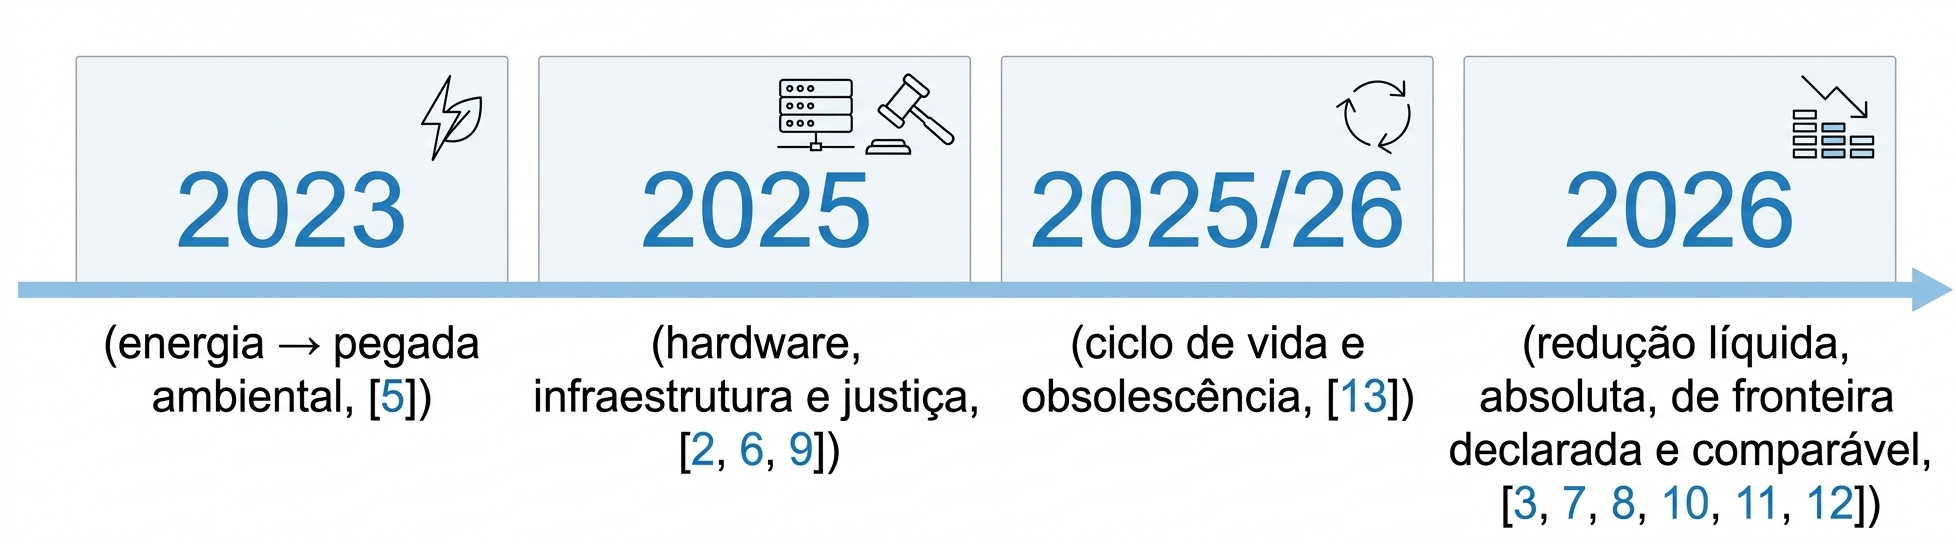
\includegraphics[width=0.85\textwidth]{linha_do_tempo.jpg}
% \caption{Evolução da definição de impacto ambiental da IA}
% \label{fig:linha}
% \end{figure}

Em síntese, a evolução conceitual deslocou o foco da mera \emph{energia de treinamento} (2023) para a ampliada de \emph{hardware, infraestrutura e justiça ambiental} (2025), avançando para a consideração do \emph{ciclo de vida completo e obsolescência} (2025/2026). Por fim, o estado atual exige que qualquer métrica de \emph{redução seja líquida, absoluta, fundamentada em fronteiras declaradas, comparável e multidimensional} (2026).

\section{Como o Impacto é Medido}

A medição do impacto ambiental da IA baseia-se predominantemente na pegada de carbono operacional: consumo energético × intensidade de carbono da rede elétrica, corrigido pelo $PUE$ do \emph{data center} \cite{2, 3, 4, 10}. Devido às diferenças na matriz energética local, a mesma carga computacional pode gerar emissões de 5 a 30 vezes distintas conforme a região \cite{2, 3, 4}. Os instrumentos de avaliação dividem-se em três famílias: estimadores baseados em tempo e potência nominal ($TDP$); monitores em tempo de execução via \emph{telemetria} de hardware (coleta de dados do equipamento), como RAPL e NVML; e Avaliação do Ciclo de Vida ($ACV$) \cite{1, 4, 10, 11}. Destacam-se as ferramentas CodeCarbon, Carbontracker, eco2AI e Experiment Impact Tracker \cite{1, 4, 10, 11}. Para o consumo hídrico, utiliza-se o $WUE$ (\emph{Water Usage Effectiveness}), que distingue o uso local (refrigeração direta) do uso fora do local (geração de eletricidade na rede) \cite{10, 12}.

Um ponto crítico enfatizado nas revisões é que indicadores indiretos (\emph{proxies}) não equivalem ao consumo energético real: métricas como $FLOPs$, quantidade de parâmetros, GPU-horas, tempo de execução e uso de memória mensuram apenas o esforço computacional ou a estrutura do modelo \cite{8, 9, 10, 11, 13}. Da mesma forma, a energia medida não equivale diretamente às emissões de carbono, e o carbono operacional não substitui uma $ACV$ completa (que inclui a fabricação e o descarte do hardware). Diante disso, em \cite{11} os autores propõem um protocolo de calibração que ajusta estimativas teóricas a medições físicas diretas (colhidas na tomada, no \emph{rack} ou via sensores internos), ressaltando que a medição direta se limita estritamente à fronteira que foi efetivamente medida.

\section{Síntese e Comparação de Técnicas}\label{sec:tecnicas}

A Tabela~\ref{tab:tecnicas} resume as técnicas por camada. Os percentuais são
os relatados pelas revisões.

\begin{table}[ht]
\centering
\caption{Técnicas de redução, resultados relatados e ressalvas}
\label{tab:tecnicas}

\scriptsize
\setlength{\tabcolsep}{3pt}
\renewcommand{\arraystretch}{0.85}

\begin{tabular}{|p{1.6cm}|p{2.5cm}|p{4.5cm}|p{3.8cm}|}
\hline
\textbf{Camada} & \textbf{Técnica} & \textbf{Resultado relatado} & \textbf{Variável medida / ressalva} \\ \hline
Dados & Modificação e aumento de dados, seleção de atributos, subamostragem & Até 92\% de energia \cite{1, 5} & Fonte única; instrumentação não descrita \\ \hline
Dados & Destilação de conjuntos de dados & 40--60\% menos iterações \cite{8} & Iterações, não energia \\ \hline
Modelo & Poda & $-$42\% \cite{3}; 20--50\% com suporte à esparsidade \cite{10} & Só rende se o hardware explora a esparsidade \\ \hline
Modelo & Quantização & $-$31\% \cite{3}; 30--60\% \cite{10}; até 94\% por operação de 32 para 8 bits \cite{4} & Por operação, inferência ou memória, conforme o estudo \\ \hline
Modelo & Destilação de conhecimento & $-$25\% \cite{3}; fator 19 \cite{2}; fator 3--5 na inferência \cite{8} & Custo do professor costuma ficar de fora \\ \hline
Modelo & Parada antecipada, ajuste de hiperparâmetros, NAS & Até 80\% \cite{2, 13}; NAS com 70--80\% menos experimentos \cite{10} & Número de experimentos e R$^2$ do preditor não são energia \\ \hline
Software & Bibliotecas de dados (Pandas, Polars, PySpark) & 60\% de potencial \cite{3}; sem percentual em \cite{7} & Benchmark dependente da carga de trabalho \\ \hline
Hardware & TPU, ASIC, FPGA & TPU 20--30\% melhor que GPU \cite{1}; 15--50$\times$ em ASICs \cite{8} & Razão de eficiência, sem carbono embutido \\ \hline
Hardware & Efeito ajustado ao ciclo de vida & $-$24,8\% cai para $-$12,3\% \cite{3} & Mostra o peso da fabricação \\ \hline
Hardware & Borda, computação em memória & $\sim$70\% menos energia de transmissão \cite{8} & Comparações pontuais; a borda desloca consumo \\ \hline
Operação & Agendamento e localização cientes de carbono & 30--50\% \cite{3}; 15--30\% \cite{8} & Reduz carbono, não necessariamente kWh \\ \hline
Operação & Refrigeração líquida e por imersão & Até $\sim$90\% (refrigeração); imersão 62,9--80\% \cite{12} & Modelado ou de fornecedor; não é a energia total \\ \hline
Operação & Serving (lotes, cache, roteamento), limite de potência & Cache $\sim$50\% de ciclos; limite de potência 12--15\% por 3\% de tempo \cite{13}; 33$\times$ por prompt em um operador \cite{12} & Uma empresa, sem auditoria independente \\ \hline
Governança & Relato, ACV, auditoria, tetos & Sem redução medida \cite{3, 7, 9, 12} & Condição de verificabilidade, não economia \\ \hline
\end{tabular}
\end{table}

\subsection{Camada de dados}


São técnicas que atuam sobre os dados e não sobre o modelo.

\textbf{1. Modificação e aumento de dados, seleção de atributos e
subamostragem.} Uma modificação no conjunto de dados é feita por meio de sua limpeza e pré-processamento. Isso elimina redundâncias, reduz o número de atributos e seleciona amostras que obedecem a esses critérios \cite{1}; o filtro dos atributos e seleção de uma subamostragem são responsáveis por remover dados que possuem baixa contribuição para o aprendizado, e há estratégias capazes de remover pontos de dados que são esperados como redundantes \cite{5}. Ademais, é útil aumentar o número de dados, gerando versões alteradas dos exemplos que já existem com o objetivo de melhorar a generalização e reduzir a coleta e rotulação de mais dados; a principal desvantagem desse método é que ele pode introduzir variações nas predições e reduzir a acurácia \cite{1}. Essas técnicas têm por objetivo reduzir o treinamento e, consequentemente, seu custo, utilizando menos dados e dados melhores.

\textbf{2. Destilação de conjuntos de dados.} É a criação de um conjunto sintético, com menos dados, que é capaz de preservar as principais características do conjunto original \cite{1}. O treinamento do modelo é feito utilizando essa representação reduzida, o que diminui o número de iterações de treinamento (entre 40 a 60 por cento a menos nos estudos feitos) \cite{8}. É importante ressaltar que há custo para construir o conjunto destilado; esse custo deve entrar no balanço, e nem sempre o ganho em iterações é transformado em ganho energético.

\subsection{Camada de modelo}

São técnicas que atuam diretamente nos modelos.

\textbf{3. Poda.} É usada para remover parâmetros ou estruturas que têm baixa contribuição. Existem três tipos de poda (não estruturada, estruturada e dinâmica): a poda não estruturada elimina pesos de forma individual, geralmente aqueles com valor próximo de zero; a estruturada pode eliminar neurônios, canais ou camadas inteiras, o que é mais amigável para o hardware; a dinâmica é uma poda feita durante o treinamento \cite{4, 13}. Ademais, existe a busca de sub-redes, mais eficazes, por \emph{lottery tickets} e \emph{rewinding}, o que evita fazer várias rodadas de poda e retreinamento \cite{13}. O ganho econômico é possível pela redução das operações e dos acessos à memória, entretanto, só é efetivo se o hardware for capaz de explorar a esparsidade resultante \cite{10}. Em contrapartida, é possível ter perdas na acurácia e no retreinamento.

\textbf{4. Quantização.} É utilizada para reduzir a precisão numérica usada para representar pesos, por exemplo, de 32 bits (FP32) para INT8 ou INT4 \cite{4, 10, 13}. Existem duas abordagens possíveis: a quantização pós-treinamento, que é mais barata e que utiliza calibração com amostras representativas; o treinamento consciente da quantização, que é responsável por simular uma baixa precisão durante o treino, preservando a melhor acurácia \cite{4, 13}. O menor número de bits diminui o volume de dados que trafega na memória e gera contas aritméticas mais baratas \cite{4}. A economia depende do hardware suportar operações de baixa precisão e de que a acurácia seja preservada \cite{10, 13}.

\textbf{5. Destilação de conhecimento.} É a utilização de um modelo professor grande, isto é, um modelo já treinado que transfere seu comportamento a um modelo aluno menor, usado na inferência \cite{1, 4}. O modelo professor é capaz de fornecer probabilidades suaves e a transferência de comportamento pode ser calcada em resposta, em características intermediárias ou nas relações entre as amostras \cite{4}. Isso faz com que o aluno exija menos memória e cálculo por resposta, o que é acumulado em milhões de inferências \cite{4}. Em contrapartida, a eficiência depende de ter um professor qualificado e do custo de treinamento do professor e do aluno \cite{4, 8}.

\textbf{6. Parada antecipada, ajuste de hiperparâmetros e NAS.} São técnicas que reduzem o custo da \emph{busca} pelo modelo. A parada antecipada é útil para interromper treinamentos quando o ganho em desempenho se estabiliza ou atinge um limiar, o que evita novos ciclos de treinamento sem ganho \cite{2}, o que também possibilita o descarte de candidatos que possuem baixo desempenho na otimização de hiperparâmetros \cite{13}. No ajuste bayesiano, são usados modelos probabilísticos capazes de explorar o espaço de hiperparâmetros que possuem menos avaliações \cite{2}. A busca de arquiteturas neurais (NAS) é responsável por automatizar a escolha de topologias que combinam qualidade, FLOPs, memória, latência e energia, e utiliza preditores capazes de rejeitar arquiteturas antes do treinamento completo \cite{10,13}. É importante contabilizar tanto o custo do preditor quanto o de toda a busca.

\subsection{Camada de software}

São técnicas que atuam a nível de software.

\textbf{7. Bibliotecas de dados.} É feita uma intervenção na fase de preparação e movimentação dos dados, isto é, antes do modelo, ao escolher entre bibliotecas como Pandas, Polars e PySpark, que são responsáveis por organizar paralelismo, memória e a execução de formas diferentes \cite{3, 7}. O método identificado é o \emph{benchmark}, que faz um comparativo de tempo, carga de CPU e energia \cite{7}. A mesma ideia surge quando há comparações entre \emph{frameworks} de aprendizado profundo; entretanto, as revisões divergem em qual é mais eficiente em treino e em inferência \cite{4, 5}. A escolha da biblioteca vencedora depende do contexto, não tendo uma que vença todos \cite{7}.


\subsection{Camada de hardware} % 5.4
% Seção já ajustada
Nessa camada aborda estratégias de uso de hardware especializado motiva redução da marca de carbono.

\textbf{8. Processadores ASIC e FPGA.} ASICs (\textit{Application-Specific Integrated Circuits}), ou Circuitos Integrado de Aplicação Específica, dedicam circuitos e memória às operações de inteligência artificial, enquanto FPGAs (\textit{Field-Programmable Gate Array}), ou Arranjos de Portas Programável em Campo, reconfiguram a lógica e os caminhos de dados \cite{13}. Ambos os hardwares são tipos de TPUs (\textit{Tensor Processing Units}), ou  Unidade de Processamento Tensorial, processadores que executam o trabalho recorrente com mais desempenho por watt do que processadores de uso geral \cite{1, 6, 8}. O ganho real é uma razão de eficiência entre plataformas e não inclui o carbono da fabricação \cite{8} desses equipamentos, o que motiva a próxima linha.

\textbf{9. Efeito ajustado ao ciclo de vida.} É uma forma de avaliar o hardware e sua eficiência operacional em relação ao carbono da fabricação, amortizado pela vida útil do equipamento (emissão de fabricação $\times$ número de unidades $\times$ fração de amortização) \cite{3}. Esse efeito agrupado do hardware cai de $-$24,8\% para $-$12,3\%, porque são necessários de 2 a 5 anos de economia operacional para compensar a fabricação \cite{3}. A avaliação do ciclo de vida dessas TPUs com uma métrica de computação da intensidade de carbono é um exemplo de aplicação \cite{7}.

\textbf{10. Borda e computação em memória.} A computação de borda é o onde acontece o processamento dos dados próximo de onde são gerados, o que ameniza a transmissão contínua à nuvem (cerca de 70\% menos energia de transmissão) \cite{8, 10}. A computação em memória e processamento em memória aproximam as operações para perto da memória com objetivo de melhorar o tráfego entre processador e memória, com ganhos que vão de centenas de vezes a milhares em comparações específicas \cite{10, 13}. Assim, como a borda desloca consumo e fabricação para os dispositivos locais, essa descentralização altera os impactos incorporados \cite{8}.

\subsection{Camada de operação} % 5.5
%Refinado
Nessa seção, trazemos estratégias sobre planejamento de horário para uso, refrigeração por líquidos e otimização da execução dos modelos.

\textbf{11. Agendamento e localização cientes de carbono.} Observar como tarefas flexíveis no tempo, para janelas de maior oferta de energia renovável, e no espaço, para
regiões de distribuição com fontes mais limpas \cite{3, 8, 11} pode ser uma boa estratégia. Nesse sentido, observamos mais o carbono por kWh e não sobre o kWh consumido \cite{3}. No entanto, necessita-se considerar prazos e níveis de serviço, custos de migração de dados e de pausa e retomada (\emph{checkpointing}) \cite{11,
13}, além do risco de ``vazamento de carbono'', quando o treinamento dos modelos aproveitou mais de energia limpa, ao passo que a execução do serviço usou mais de rede fóssil \cite{3}. Além disso, devemos considerar que esses \textit{datacenters} dissipam muito calor.

\textbf{12. Refrigeração líquida e por imersão.} Essa estratégia é considerar a refrigeração desses servidores com líquido em vez de ar, onde a refrigeração direta ao chip possuiria líquido circulante junto ao componente,
e em uma configuração para imersão monofásica, os componentes ficam mergulhados em fluido \cite{10, 12}.
Os indicadores de eficiência de uso de energia e de uso de água observam como a refrigeração evaporativa, por exemplo,
reduz energia de refrigeração, mas eleva o consumo de água \cite{12}. Assim, os ganhos relatados vêm de simulação, pilotos e dados de fornecedores, mas não são a energia
total do data center e deixam de fora fluidos, fabricação e manutenção \cite{12}. 

\textbf{13. Serving e limite de potência.} Talvez uma das melhores estratégias pensadas pode ser otimizar a fase de inferência (\textit{serving}) em ambiente de produção. A etapa de inferência de inteligência artificial combina os agrupamentos de requisições (lotes), cache de
resultados e ativações, roteamento entre hardware heterogêneo e multi-locação para preencher ciclos ociosos \cite{13} de uso. Enquanto isso, o limite de potência (\emph{power capping}) impõe um teto de consumo e troca energia por tempo, com 12--15\% menos energia e 3\% mais tempo de conclusão \cite{11, 13}. Portanto, o resultado de 33$\times$ por \emph{prompt} vem de um único operador, combina melhorias do modelo e da utilização e não foi auditado de forma independente \cite{12}.

\subsection{Camada de governança} % 5.6
%Refinado
Nessa camada, observamos três aspectos de observabilidade de medições e fiscalizações da operação e treinamento de inteligência artificial.

\textbf{14. Relato, Avaliação do Ciclo de Vida, auditoria e tetos.} Abordar possíveis reduções verificáveis. Propondo mecanismos como o relato obrigatório em cinco categorias de divulgação e três níveis de conformidade (Protocolo de Contabilização de Carbono para IA Sustentável) \cite{3}, a divulgação auditada e a certificação independente para sistemas acima de um limiar de computação \cite{9}, Avaliação do Ciclo de Vida padronizada \cite{9}, os orçamentos de sustentabilidade que limitam energia ou carbono por projeto \cite{7} e os limites absolutos de retirada de água \cite{12}. Logo, essas revisões não atribuem às medições uma  real redução, mas a transparência motiva a alteração e busca por melhores processos de decisões \cite{7, 9, 12}.

\subsection{Padrões da comparação} % 5.7
%Refinado
É notável que o maior rendimento advém dos dados (até 92\%) e da compressão de modelos, e a única estimativa agregada com meta-análise é de $-$38,2\% para a otimização algorítmica, $-$24,8\% para hardware e $-$29,7\% para operação, com $-$32,4\% para o conjunto \cite{3}. Além disso, as camadas observadas atuam em fatores diferentes, quando o algoritmo reduz kWh, o hardware reduz energia por operação e a operação reduz carbono por kWh, por isso
se complementam \cite{3}. No entanto, escolher o algoritmo mais simples que resolve a tarefa também é uma redução considerável, pois modelos clássicos gastam muito menos energia que àqueles que usam arquiteturas Transformers \cite{2}. Assim, Khan et al. recomendam esgotar primeiro a compressão algorítmica e só depois o hardware \cite{3}.

\section{Análise Crítica e Gargalos}\label{sec:gargalos} % 6

\subsection{Gargalos de medição} % 6.1

Há uma inconsistência entre as fronteiras; as estimativas variam de acordo com o que entra na conta; a maioria dos estudos não leva em conta a inferência e não leva em conta o carbono embutido \cite{3}. Além disso, existe uma diferença na medição da intensidade média anual e na marginal da rede, e uma diferença na alocação em nuvem multiusuário \cite{3}. Muitos trabalhos não discutem sobre hardware ou intervalos de confiança \cite{3, 8}, e somente alguns estudos disponibilizam ferramentas \cite{5}. Em muitos casos, proxies são tratados como energia \cite{2, 4, 5}.

\subsection{Gargalos de evidência}

Muitos resultados usam metodologias conhecidas \cite{1,2,4,5,8}. Dessa forma, os melhores dados vêm de operadores, que não são auditáveis; a economia de refrigeração é, em sua maioria, modelada ou de fornecedores \cite{12}. Existem inconsistências internas e entre as revisões, como sentido invertido na comparação PyTorch e TensorFlow \cite{4, 5} e o peso relativo no treinamento e inferência \cite{1}. Os \emph{frameworks} propostos em \cite{6, 7, 11} não foram validados de forma empírica.

\subsection{Gargalos conceituais}

Um dos problemas é o efeito rebote, que pode anular ganhos por tarefa \cite{3, 6, 7, 8}. Além disso, há o deslocamento de impacto, isto é, a energia de baixo carbono pode gerar o aumento na intensidade hídrica \cite{10, 12}, a borda desloca o consumo e a fabricação \cite{8}, e o treinamento usando energia limpa para servir em rede fóssil gera ''vazamento de carbono'' \cite{3}. A maioria das técnicas utilizadas possui custos ocultos \cite{8,10,13}, e o ganho operacional de hardware eficiente pode ser reduzido pelo carbono de fabricação \cite{3, 8}. Existem também impedimentos práticos, como o alto investimento monetário e prazos longos para hardware \cite{3}, e falta na cobertura de água, materiais e no fim de vida \cite{8,11,12}.


\section{Propostas Futuras}\label{sec:futuro}

As propostas futuras estruturam-se em eixos de avaliação e mitigação. Na medição, em \cite{3} e \cite{10} os autores recomendam relatos obrigatórios em camadas, enquanto em \cite{6} sugere-se a métrica de kgCO$_2$e por hora de inferência. Em \cite{4} e \cite{11} destaca-se o uso de \emph{benchmarks} e a calibração de estimadores contra medições físicas. Para o ciclo de vida, em \cite{3, 5, 8, 9, 11} reforça-se o uso da ACV (ISO 14040/44) abrangendo fabricação, água e circularidade. Para viabilizar essas práticas, em \cite{3, 5, 12} os autores demandam estudos reprodutíveis, atribuição exata de ganhos, medições independentes de refrigeração e análises hídricas expandidas.

Em relação à governança, em \cite{9} os autores propõem certificações independentes e a divulgação auditada para modelos que ultrapassem 10$^{18}$ FLOPs. Sugerem-se ainda tetos absolutos de emissão \cite{3}, limites para a retirada de água \cite{12} e a adoção de orçamentos de sustentabilidade \cite{7}. Na infraestrutura, em \cite{6} os autores propõem alinhar a expansão da IA às estratégias de descarbonização regional (priorizando renováveis e usando reatores modulares pequenos como complemento condicional), além de integrar a carga energética da IA aos modelos climáticos globais.

No nível operacional, em \cite{4} propõe-se automatizar a seleção de técnicas e incorporar o carbono como objetivo na Busca de Arquiteturas Neurais (NAS). Em \cite{10} e \cite{13} os autores recomendam \emph{hardware} neuromórfico, computação em memória e modelos especializados por domínio. Em \cite{10} e \cite{11} reforça-se o agendamento de tarefas sensível às emissões de carbono e à disponibilidade de água. Por fim, em \cite{7} introduz-se um modelo conceitual de aprendizado por reforço multiagente, cuja recompensa penaliza as emissões operacionais e as incorporadas.

\section{Conclusão}

As treze revisões sintetizam que o impacto ambiental da IA deve ser definido
pelo ciclo de vida completo, medido com fronteiras declaradas e calibradas
contra medições reais, e reduzido por uma combinação de otimização técnica,
gestão operacional e governança. Então deixamos de economizar energia para mostrar real redução. Como a base quantitativa ainda é frágil, uma alegação de redução só é robusta se demonstrar economia líquida, para tarefa e qualidade comparáveis, com infraestrutura, ciclo de vida e escala de uso incluídos \cite{11}.

\bibliographystyle{sbc}
\bibliography{sbc-template}
\end{document}